\chapter{Thí nghiệm và Kết quả}

Tất cả thí nghiệm được thực hiện trên một GPU NVIDIA duy nhất sử dụng huấn luyện nửa chính xác (FP16) với PyTorch 2.x. Hạt giống ngẫu nhiên cố định ở 42. Kết quả trên tập kiểm tra giữ lại.

\section{So sánh Mô hình Đơn lẻ}

\begin{table}[H]
\centering
\caption{So sánh hiệu suất trên tập kiểm tra. Giá trị tốt nhất được in \textbf{đậm}.}
\begin{tabular}{lccccc}
\toprule
\textbf{Mô hình} & \textbf{Accuracy} & \textbf{Macro F1} & \textbf{AUC} & \textbf{MCC} & \textbf{Kappa} \\
\midrule
EfficientNet-B0 & \textbf{0,8836} & \textbf{0,8311} & 0,9522 & \textbf{0,7721} & \textbf{0,7710} \\
ResNet50        & 0,8603 & 0,7902 & 0,9565 & 0,7310 & 0,7309 \\
DenseNet121     & 0,8543 & 0,7967 & 0,9587 & 0,7209 & 0,7206 \\
Swin-Tiny       & 0,8490 & 0,7855 & \textbf{0,9600} & 0,7157 & 0,7150 \\
\bottomrule
\end{tabular}
\end{table}

EfficientNet-B0 dẫn đầu mọi chỉ số phân loại cứng mặc dù có ít tham số hơn mọi mô hình khác: 5,3M so với 8M (DenseNet121), 25,6M (ResNet50) và 28M (Swin-Tiny). Macro F1 của nó đạt 0,831 vượt trội ResNet50 (0,790) tới 4,1 điểm phần trăm, dù ResNet50 có gần gấp năm lần số tham số. Điều này nhất quán với giả thuyết compound-scaling của Tan và Le: tối ưu hóa đồng thời chiều sâu, chiều rộng và độ phân giải đầu vào tạo ra một biên hiệu quả khác biệt về chất lượng thay vì các lợi ích cận biên gia tăng.\footnote{Giá trị cross-entropy loss trên test (0,75) tương đối cao cho mọi mô hình là hệ quả mong đợi của Label Smoothing: các mô hình huấn luyện với target mềm ($\epsilon=0{,}1$) xuất ra độ tin cậy tối đa khoảng $1 - \epsilon + \epsilon/C \approx 0{,}93$ thay vì 1,0, tạo giá trị loss thô cao hơn mà không phản ánh sự suy giảm chất lượng phân loại.}

Một mẫu hình nổi bật khi so sánh accuracy với AUC giữa các mô hình: chúng \textbf{đảo ngược} nhau. EfficientNet-B0 dẫn đầu về các chỉ số phân loại cứng trong khi Swin-Tiny, kém 3,5 điểm phần trăm về accuracy, tạo ra AUC cao nhất (0,960). Cơ chế tự chú ý dựa trên cửa sổ của Transformer dường như tạo ra phân phối xác suất được hiệu chỉnh tốt hơn ngay cả khi các dự đoán cứng của nó kém chính xác hơn --- có thể vì việc tích hợp ngữ cảnh toàn cục pha trộn bằng chứng khắp toàn bộ tổn thương, làm mịn các ước tính tin cậy về phía tần suất lớp thực. Lợi thế calibration này không chuyển thành quyết định rời rạc tốt hơn trên 7.010 ảnh huấn luyện, nhất quán với phát hiện rằng Vision Transformer cần dữ liệu đáng kể nhiều hơn để thu hẹp khoảng cách với CNN về phân loại cứng. Trong một ứng dụng triage lâm sàng nơi output xác suất của mô hình được tiêu thụ trực tiếp cho xếp hạng rủi ro thay vì ra quyết định nhị phân, thứ tự AUC sẽ là so sánh liên quan.

\subsection{Phân tích Theo Lớp}

Melanoma (MEL) là lớp khó nhất cho mọi kiến trúc, với F1 từ 0,625 (Swin-Tiny) đến 0,695 (EfficientNet-B0). Khó khăn này có tính cấu trúc: MEL chồng lấp với BKL về sắc tố và với NV về kết cấu, cùng sự nhập nhằng làm cho melanoma khó chẩn đoán trên lâm sàng. Các giá trị AUC kể một câu chuyện đáng khích lệ hơn --- 0,913 đến 0,930 --- chỉ ra rằng các mô hình liên tục xếp hạng các trường hợp melanoma thật trên các lựa chọn lành tính ngay cả khi ngưỡng cứng 0,5 không tách được chúng. Trong một workflow triage nơi các trường hợp được sắp xếp theo điểm rủi ro thay vì gắn cờ bằng cutoff nhị phân, thứ tự xác suất này là output có giá trị.

Dermatofibroma (DF) nằm ở thái cực ngược lại: F1 từ 0,800 đến 0,938 dù chỉ có 81 mẫu huấn luyện và 17 mẫu test. Weighted Random Sampler đảm bảo Dermatofibroma xuất hiện trong mọi mini-batch thay vì bị nhấn chìm bởi NV, và đặc trưng lâm sàng riêng biệt của DF --- một tổn thương cứng giống nút bấm với các đặc điểm dermoscopy đặc trưng --- cung cấp tín hiệu phân biệt rõ ràng. Tuy nhiên, các con số này mang phương sai cao: với 17 mẫu test, một phân loại sai bổ sung dịch chuyển F1 khoảng 0,06, nên khoảng cách rõ ràng 14 điểm giữa EfficientNet-B0 (0,938) và ResNet50 (0,800) không nên được đọc như khác biệt hiệu suất đáng tin cậy.

Vascular Lesion (VASC) được phân loại tốt một cách liên tục, với AUC đạt 1,000 cho hai kiến trúc. Sắc đỏ-tím của tổn thương mạch máu cung cấp tín hiệu màu mạnh, rõ ràng mà mọi mô hình đều nhận diện đáng tin cậy. Cũng như DF, tập test 22 mẫu nghĩa là các con số riêng lẻ có nhiễu, nhưng các giá trị AUC gần hoàn hảo ổn định qua các kiến trúc và phản ánh độ rõ ràng thị giác của lớp này.

\subsection{Động lực Huấn luyện}

\begin{figure}[H]
\centering
\begin{subfigure}{\textwidth}
    \makebox[\textwidth][c]{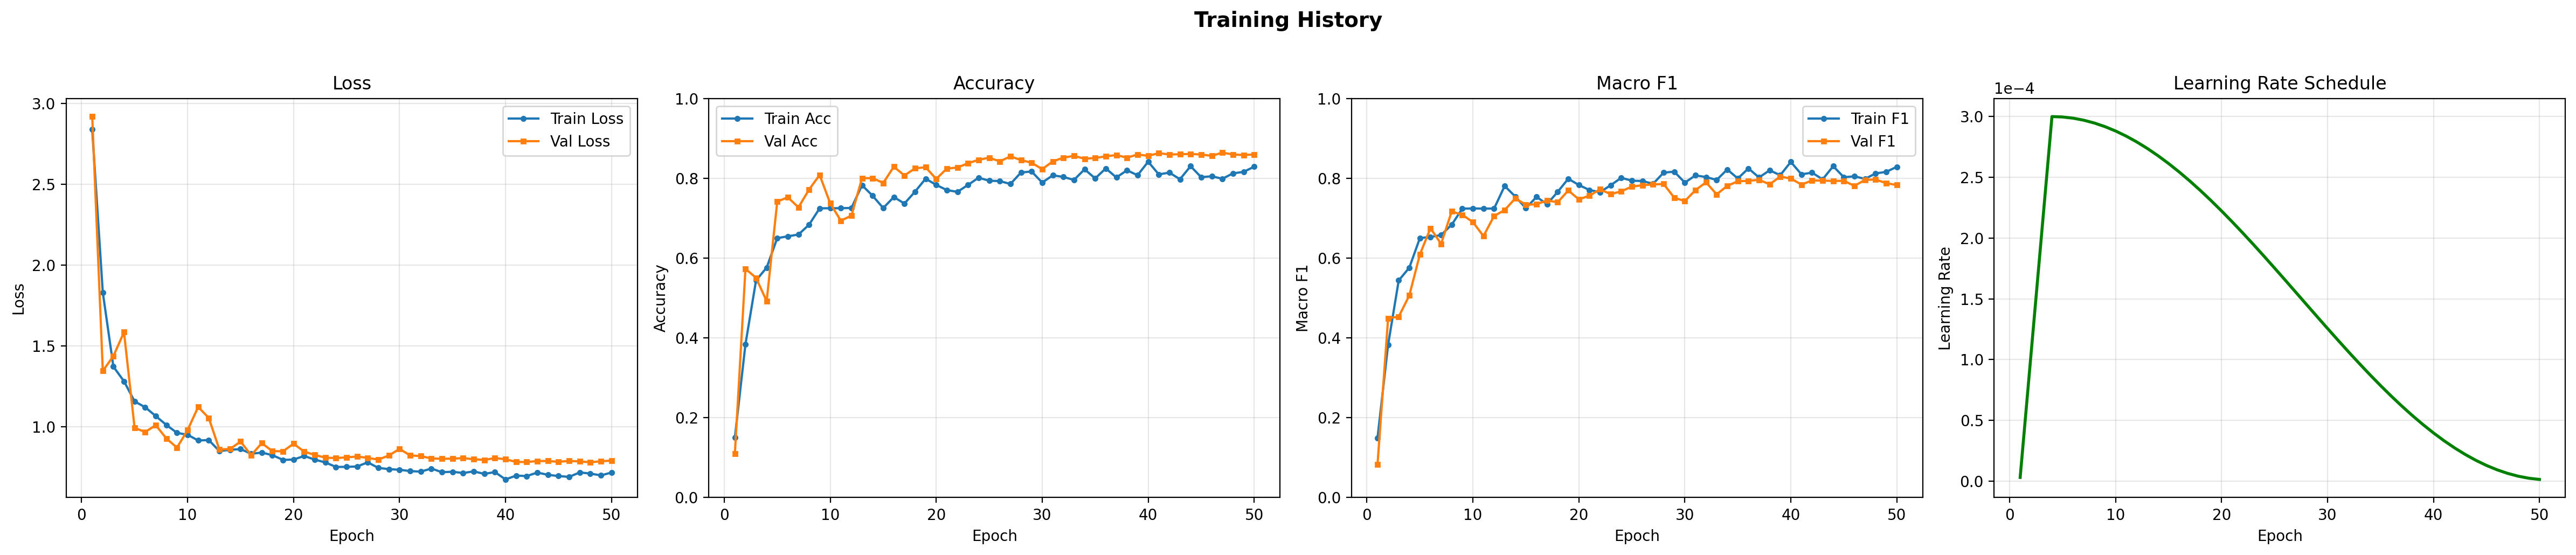
\includegraphics[width=1.15\textwidth]{figures/eb0_training_history.png}}
    \caption{EfficientNet-B0}
\end{subfigure}
\vspace{0.6cm}
\begin{subfigure}{\textwidth}
    \makebox[\textwidth][c]{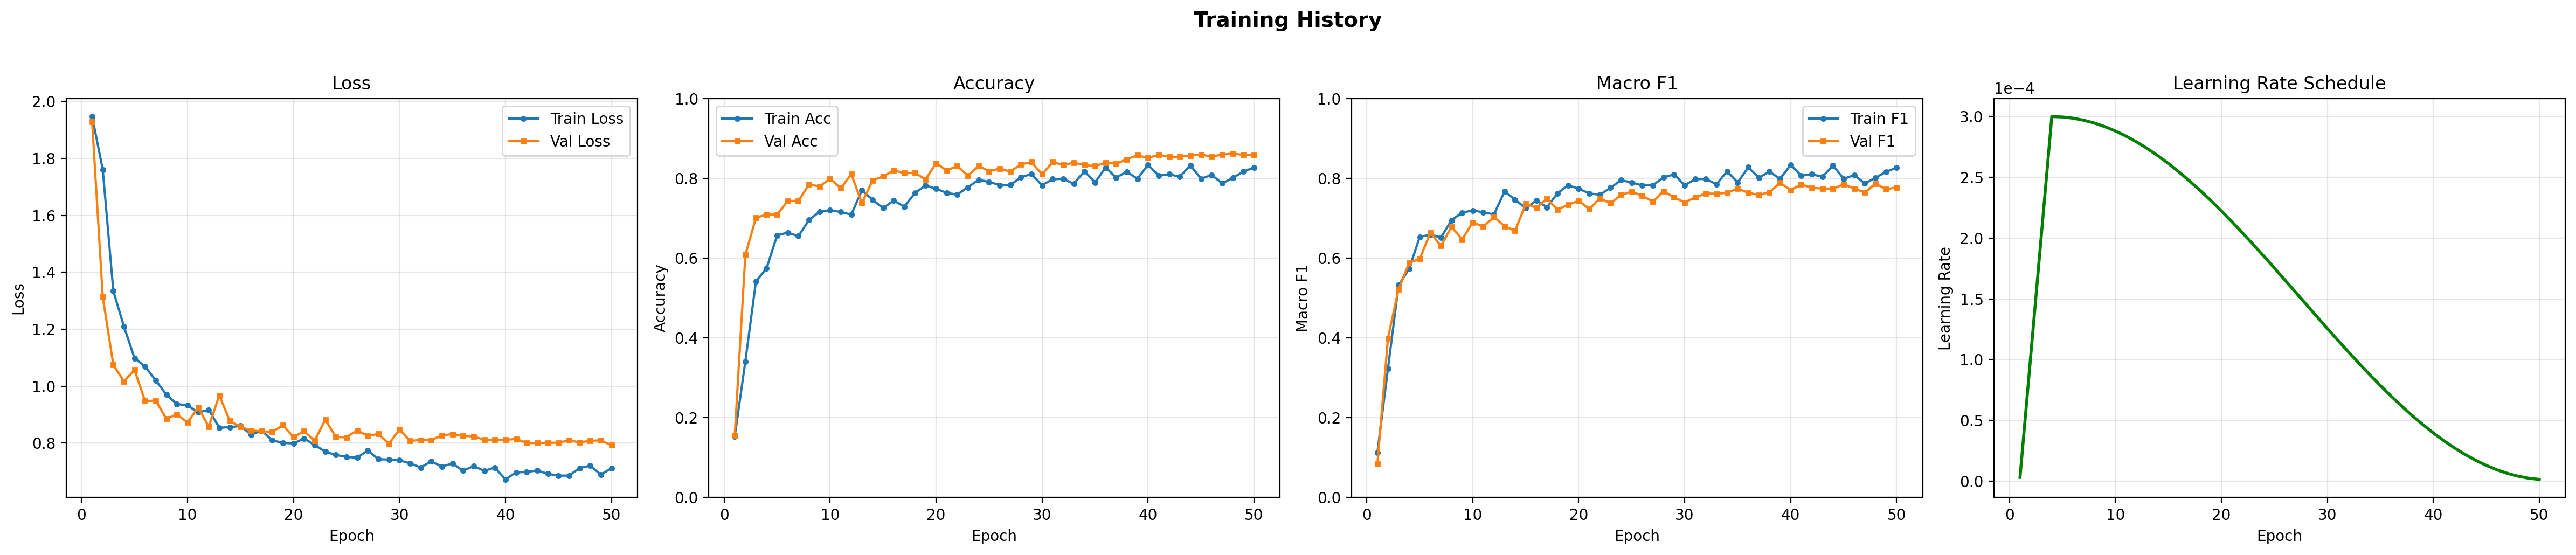
\includegraphics[width=1.15\textwidth]{figures/rn50_training_history.png}}
    \caption{ResNet50}
\end{subfigure}
\caption{Lịch sử huấn luyện: loss, accuracy và tốc độ học qua các epoch.}
\end{figure}

\begin{figure}[H]
\centering
\begin{subfigure}{\textwidth}
    \makebox[\textwidth][c]{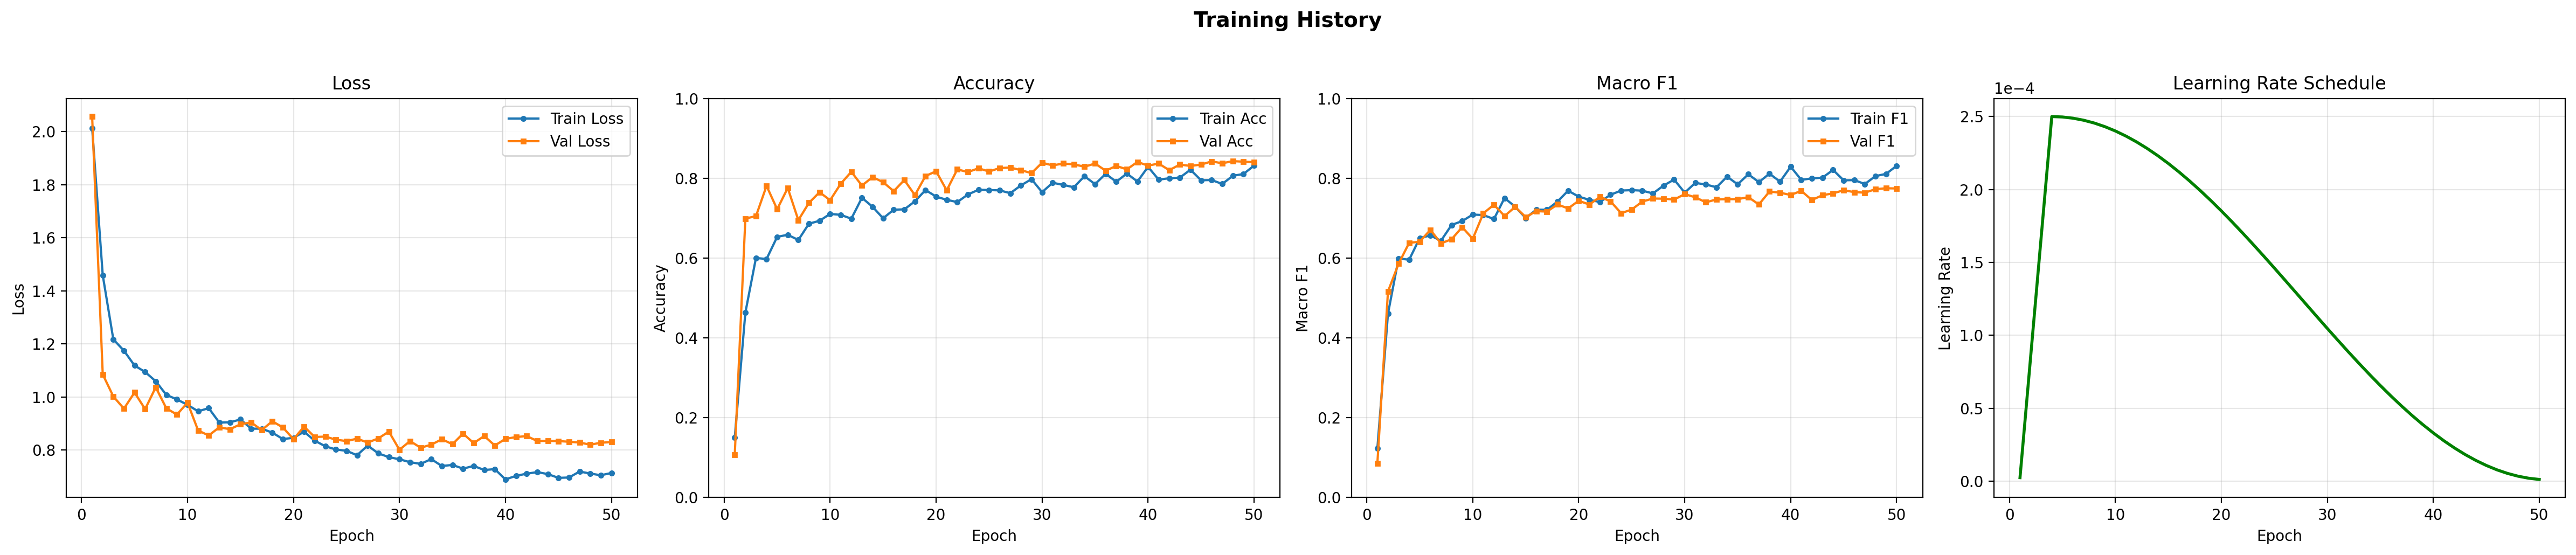
\includegraphics[width=1.15\textwidth]{figures/dn121_training_history.png}}
    \caption{DenseNet121}
\end{subfigure}
\vspace{0.6cm}
\begin{subfigure}{\textwidth}
    \makebox[\textwidth][c]{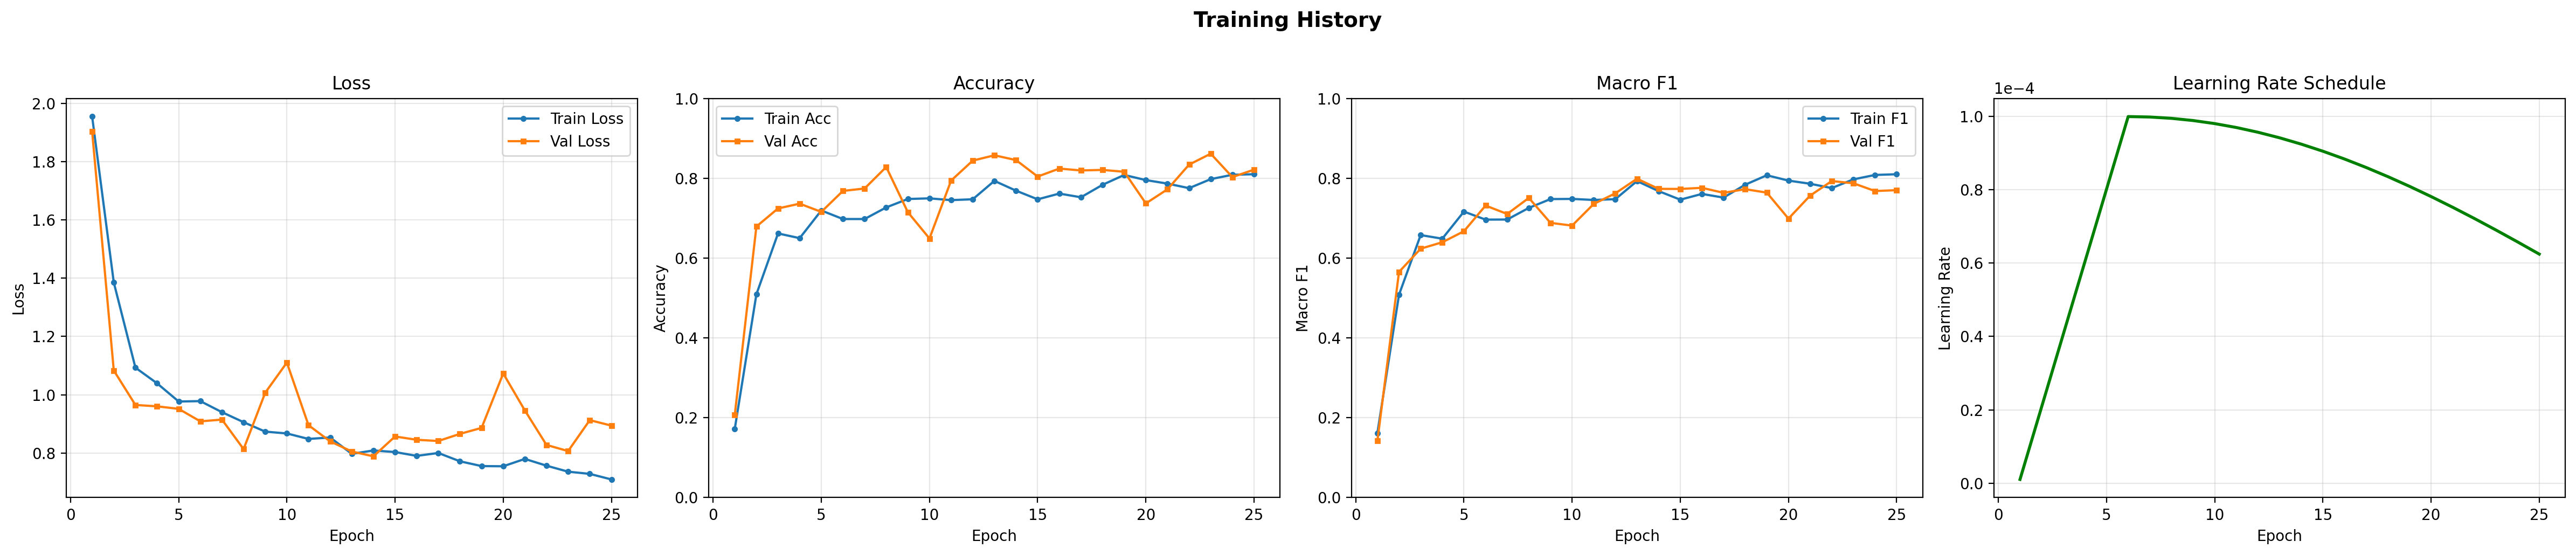
\includegraphics[width=1.15\textwidth]{figures/swin_training_history.png}}
    \caption{Swin-Tiny}
\end{subfigure}
\caption{Lịch sử huấn luyện (tiếp theo).}
\end{figure}

Tốc độ hội tụ khác nhau giữa các kiến trúc theo cách nhất quán với các tính chất đã biết của mỗi thiết kế:
\begin{itemize}
    \item EfficientNet-B0 và ResNet50 đều đạt đỉnh tại epoch 39, với dừng sớm kích hoạt sau 12 epoch tiếp theo không cải thiện.
    \item DenseNet121 đạt checkpoint tốt nhất tại epoch 49 trên 50, phản ánh xu hướng của các mạng có kết nối dày đặc cải thiện dần qua nhiều epoch khi mô hình kết nối dày đặc khai thác đầy đủ việc tái sử dụng đặc trưng.
    \item Swin-Tiny kích hoạt dừng sớm tại epoch 25 (tốt nhất tại epoch 13), tốc độ hội tụ nhanh nhất nhưng cũng là plateau sớm nhất. Điều này nhất quán với việc các mô hình Transformer dễ quá khớp hơn trên tập dữ liệu nhỏ --- warmup 5 epoch và weight decay cao hơn (0,05) làm chậm sự hội tụ ban đầu nhưng không thể bù đắp đầy đủ cho yêu cầu dữ liệu.
\end{itemize}

Tất cả các mô hình hội tụ mà không quá khớp đến mức cần can thiệp --- loss validation theo dõi loss huấn luyện xuyên suốt, xác nhận rằng tổ hợp các kỹ thuật điều chuẩn (Mixup, CutMix, Label Smoothing, Weight Decay) là đủ để ngăn sự sụp đổ về lớp đa số xuất hiện khi không có chúng.

\subsection{Ma trận Nhầm lẫn}

\begin{figure}[H]
\centering
\begin{subfigure}{\textwidth}
    \makebox[\textwidth][c]{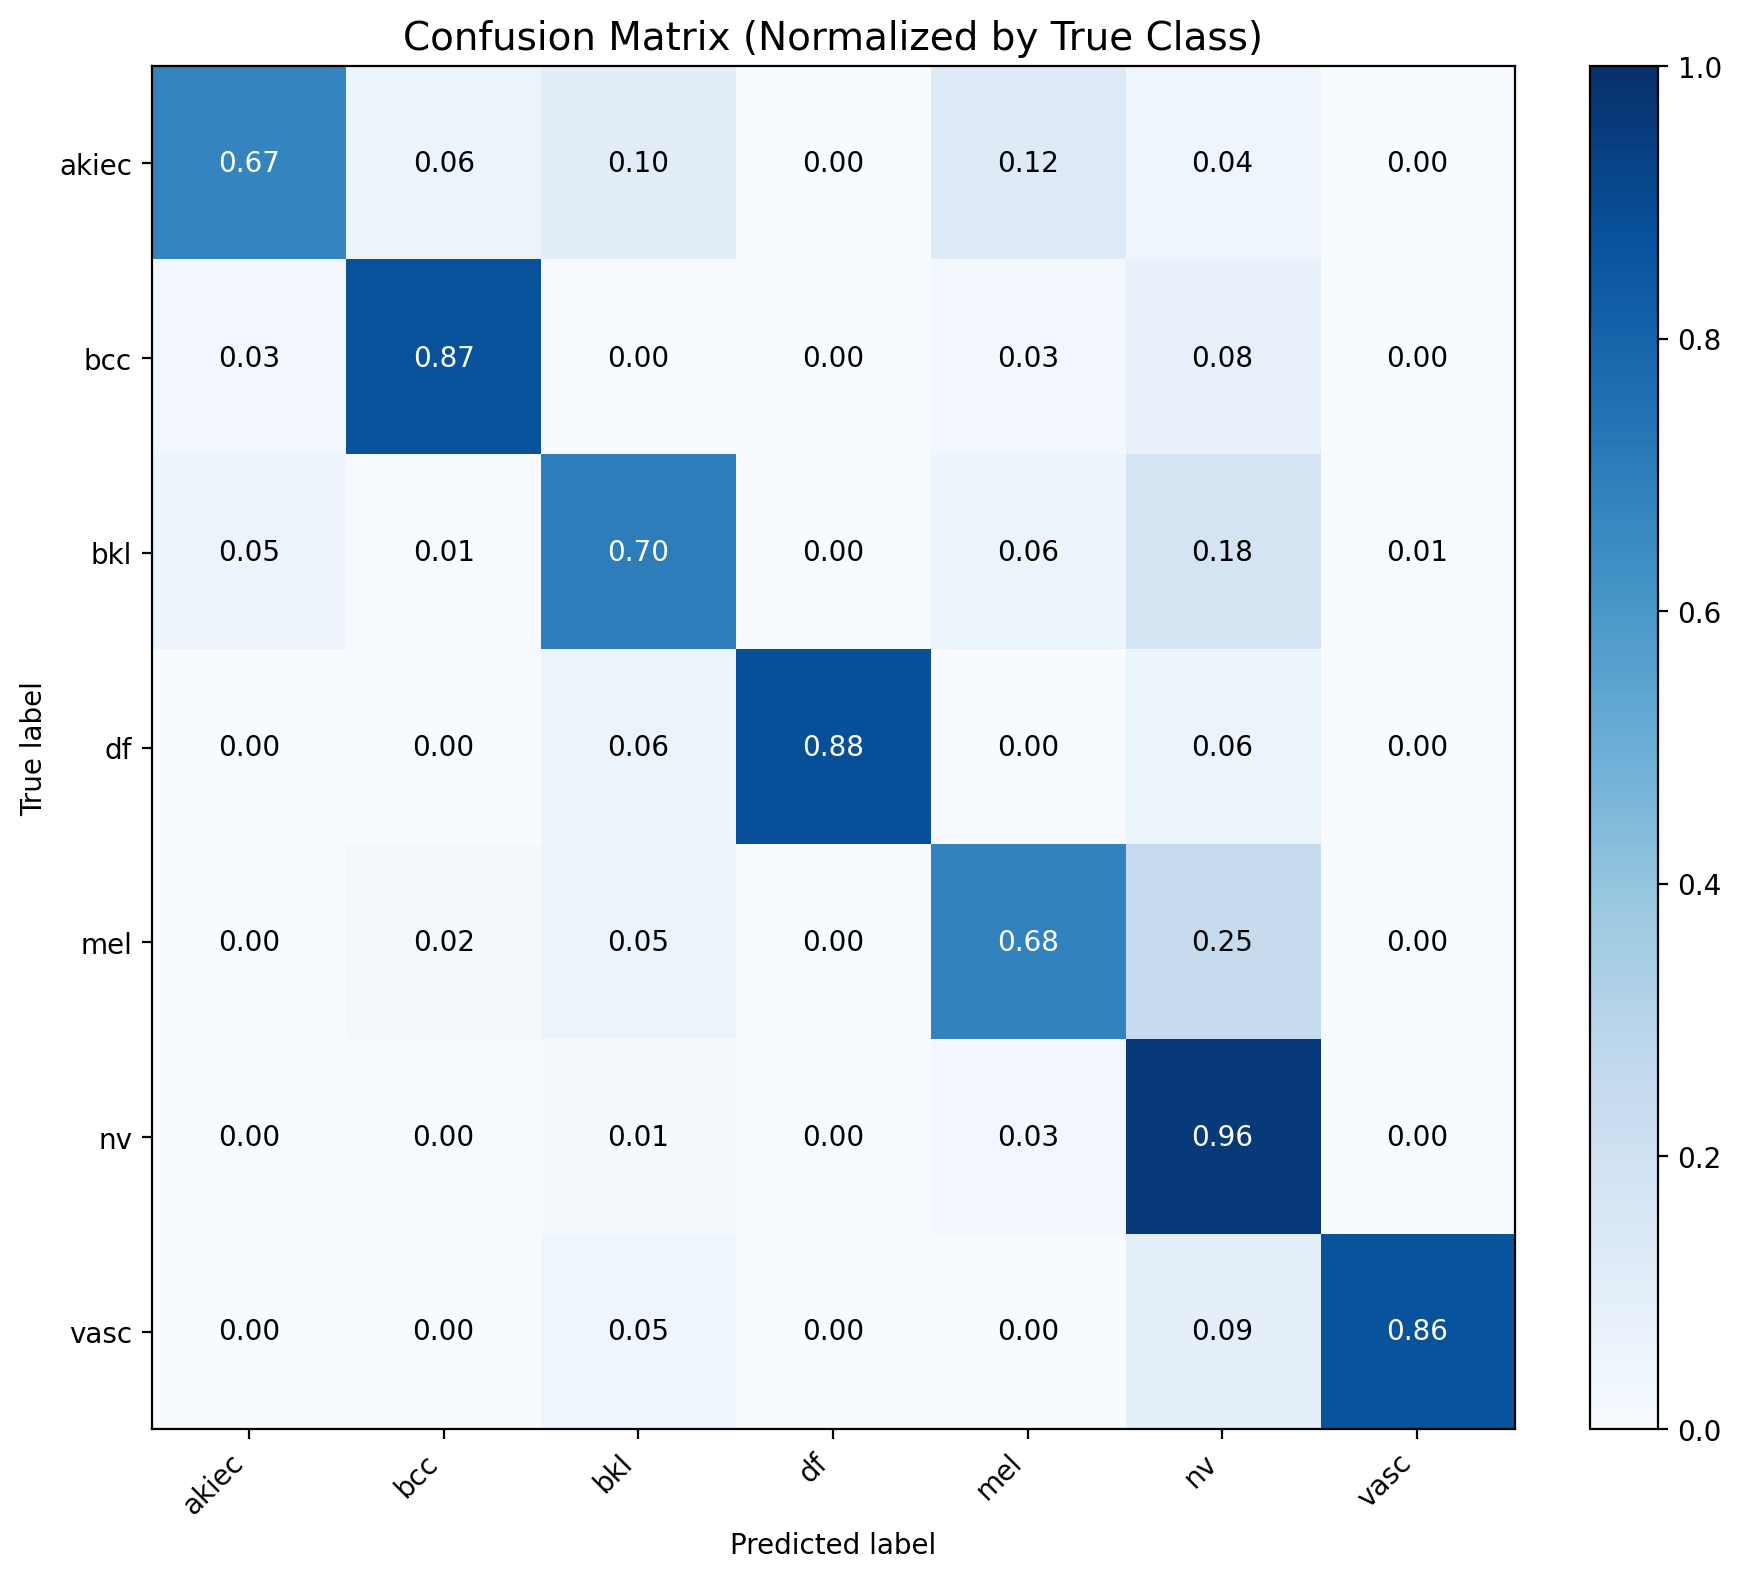
\includegraphics[width=0.9\textwidth]{figures/eb0_confusion_matrix.png}}
    \caption{EfficientNet-B0}
\end{subfigure}
\vspace{0.6cm}
\begin{subfigure}{\textwidth}
    \makebox[\textwidth][c]{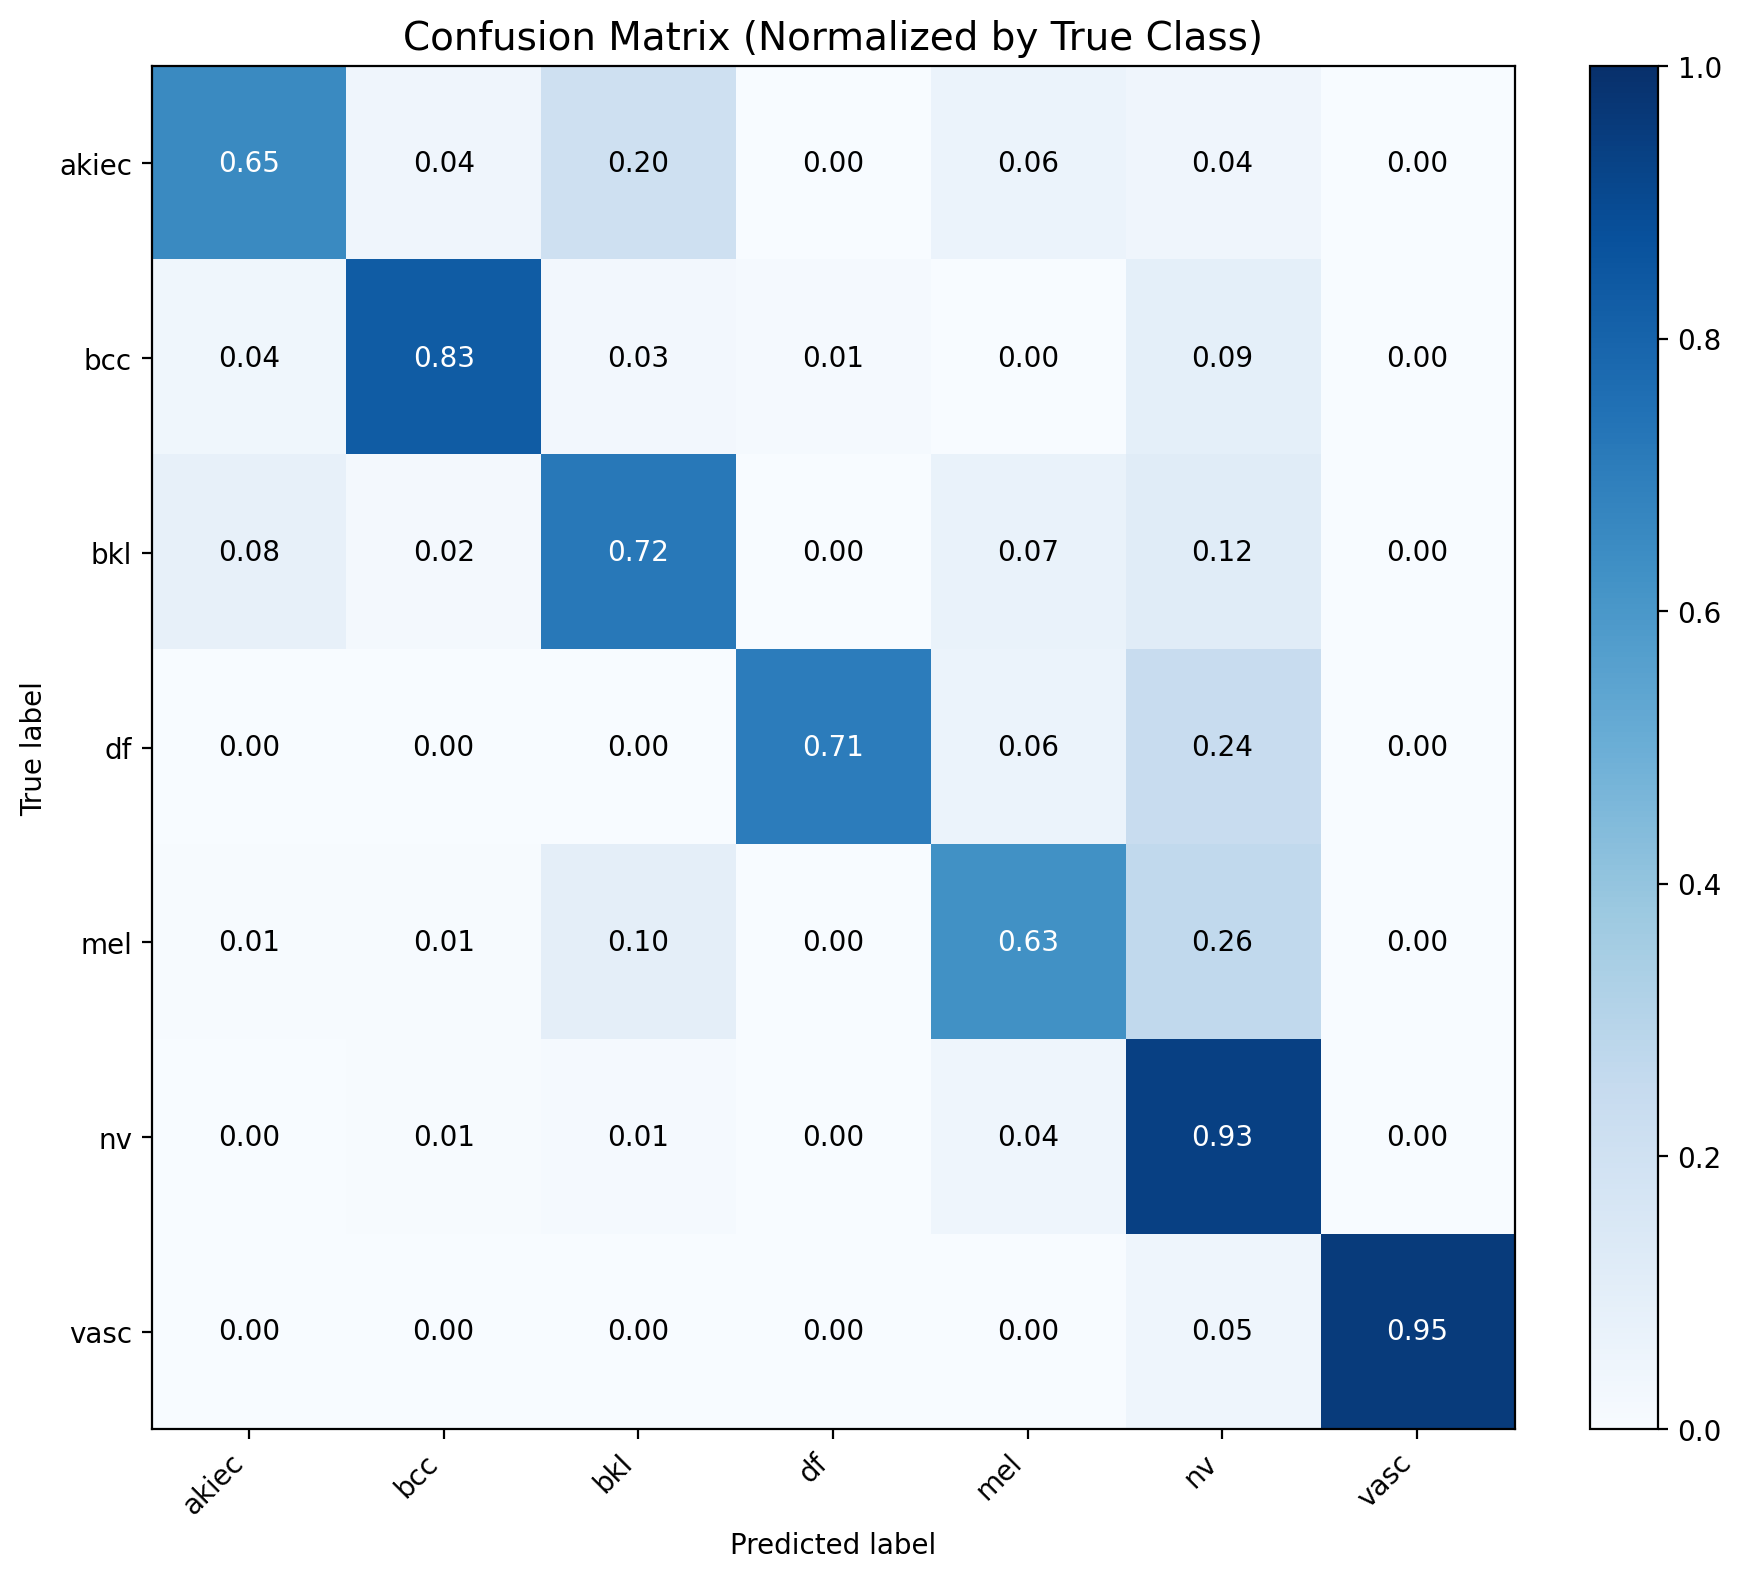
\includegraphics[width=0.9\textwidth]{figures/rn50_confusion_matrix.png}}
    \caption{ResNet50}
\end{subfigure}
\caption{Ma trận nhầm lẫn chuẩn hóa trên tập kiểm tra.}
\end{figure}

\begin{figure}[H]
\centering
\begin{subfigure}{\textwidth}
    \makebox[\textwidth][c]{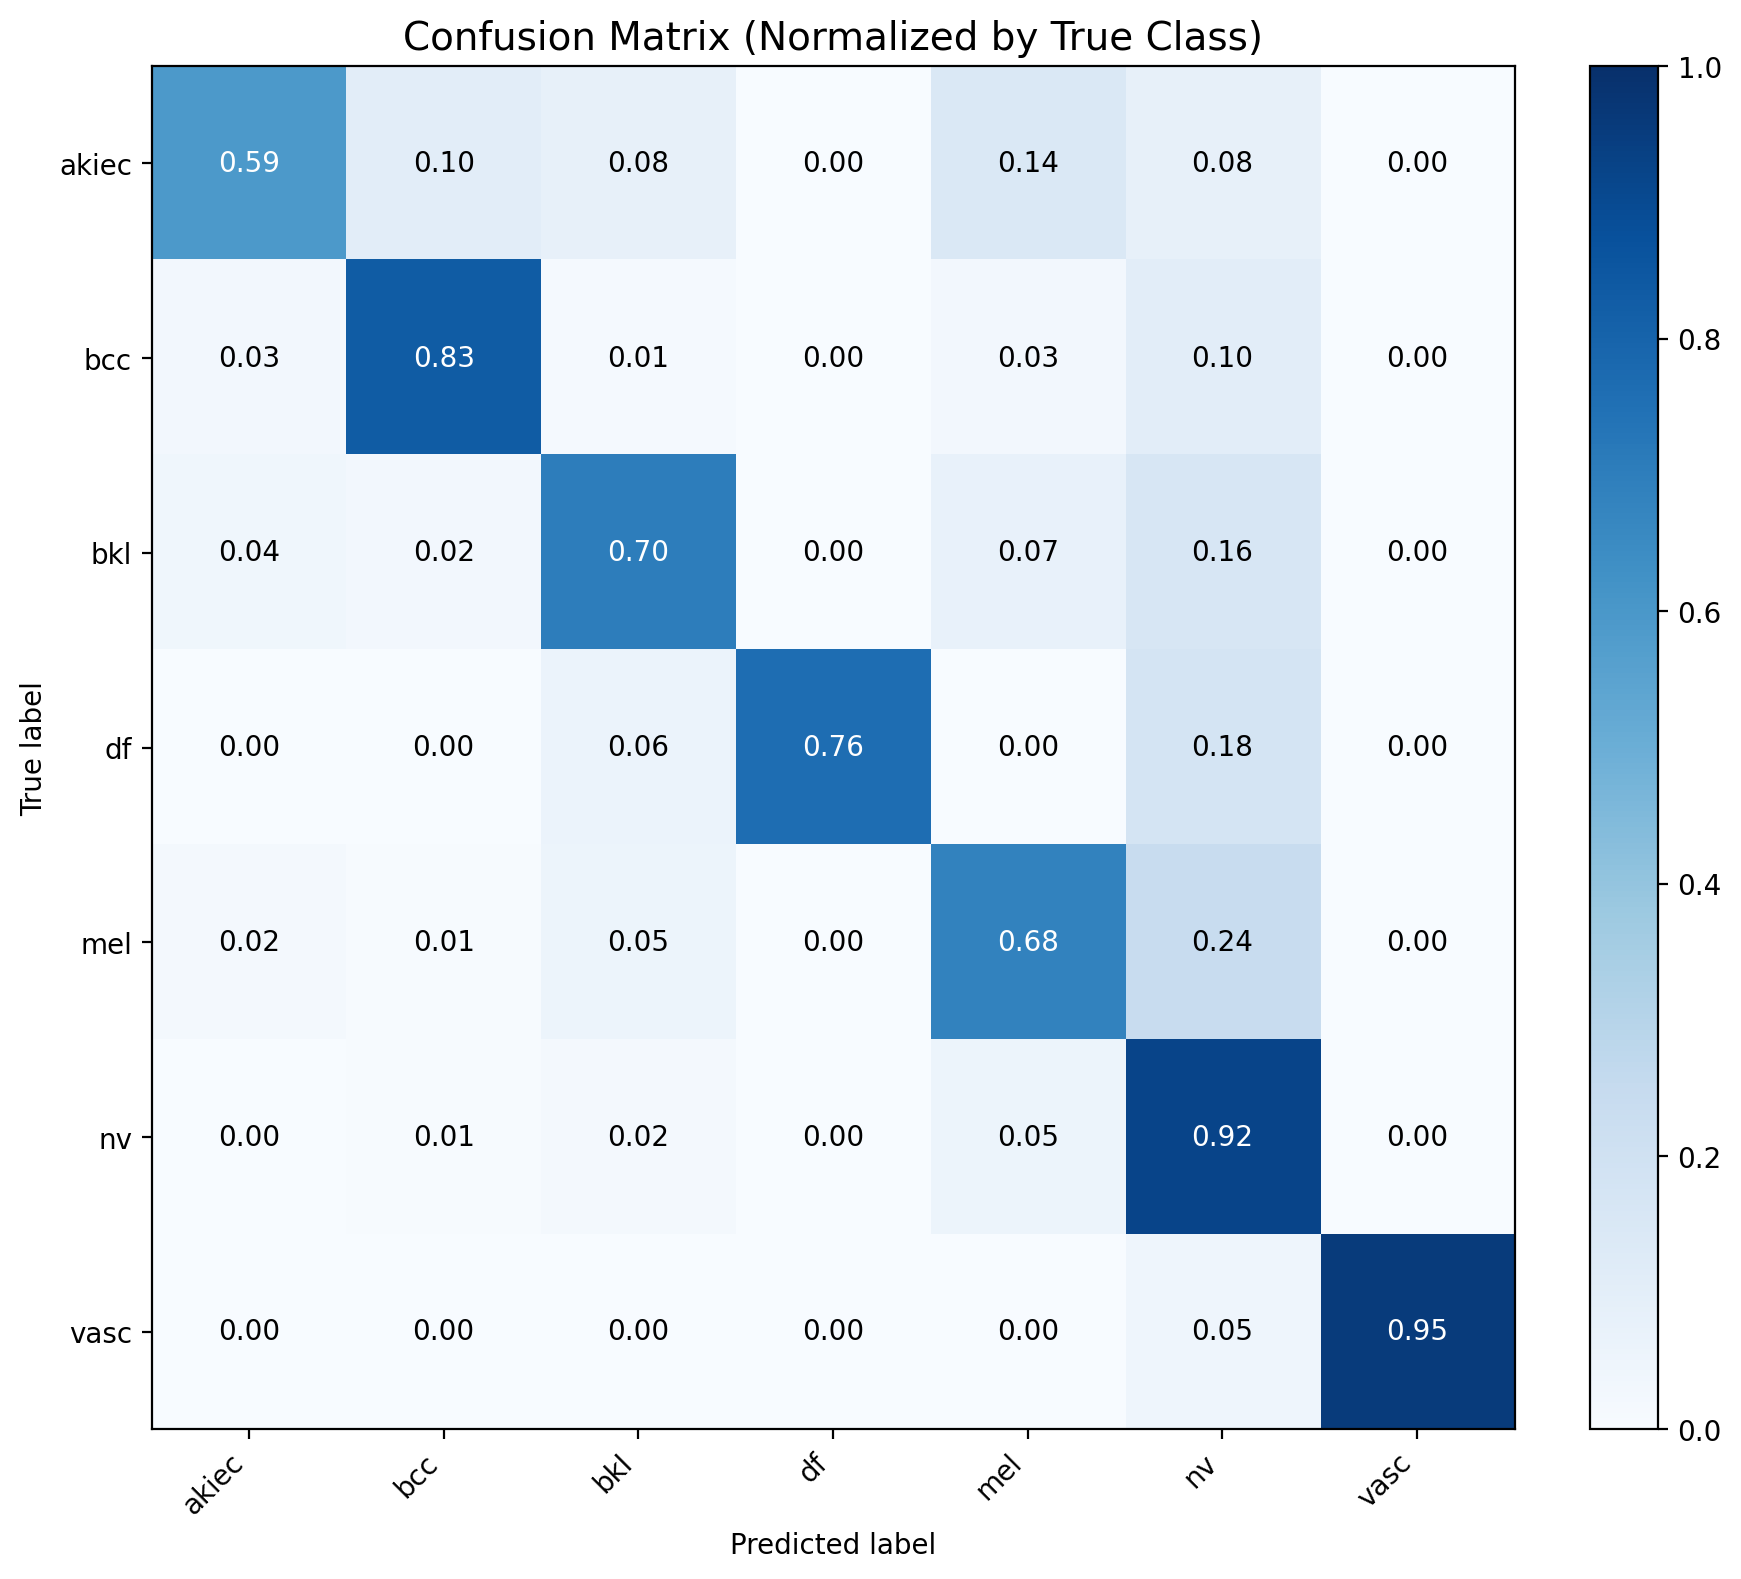
\includegraphics[width=0.9\textwidth]{figures/dn121_confusion_matrix.png}}
    \caption{DenseNet121}
\end{subfigure}
\vspace{0.6cm}
\begin{subfigure}{\textwidth}
    \makebox[\textwidth][c]{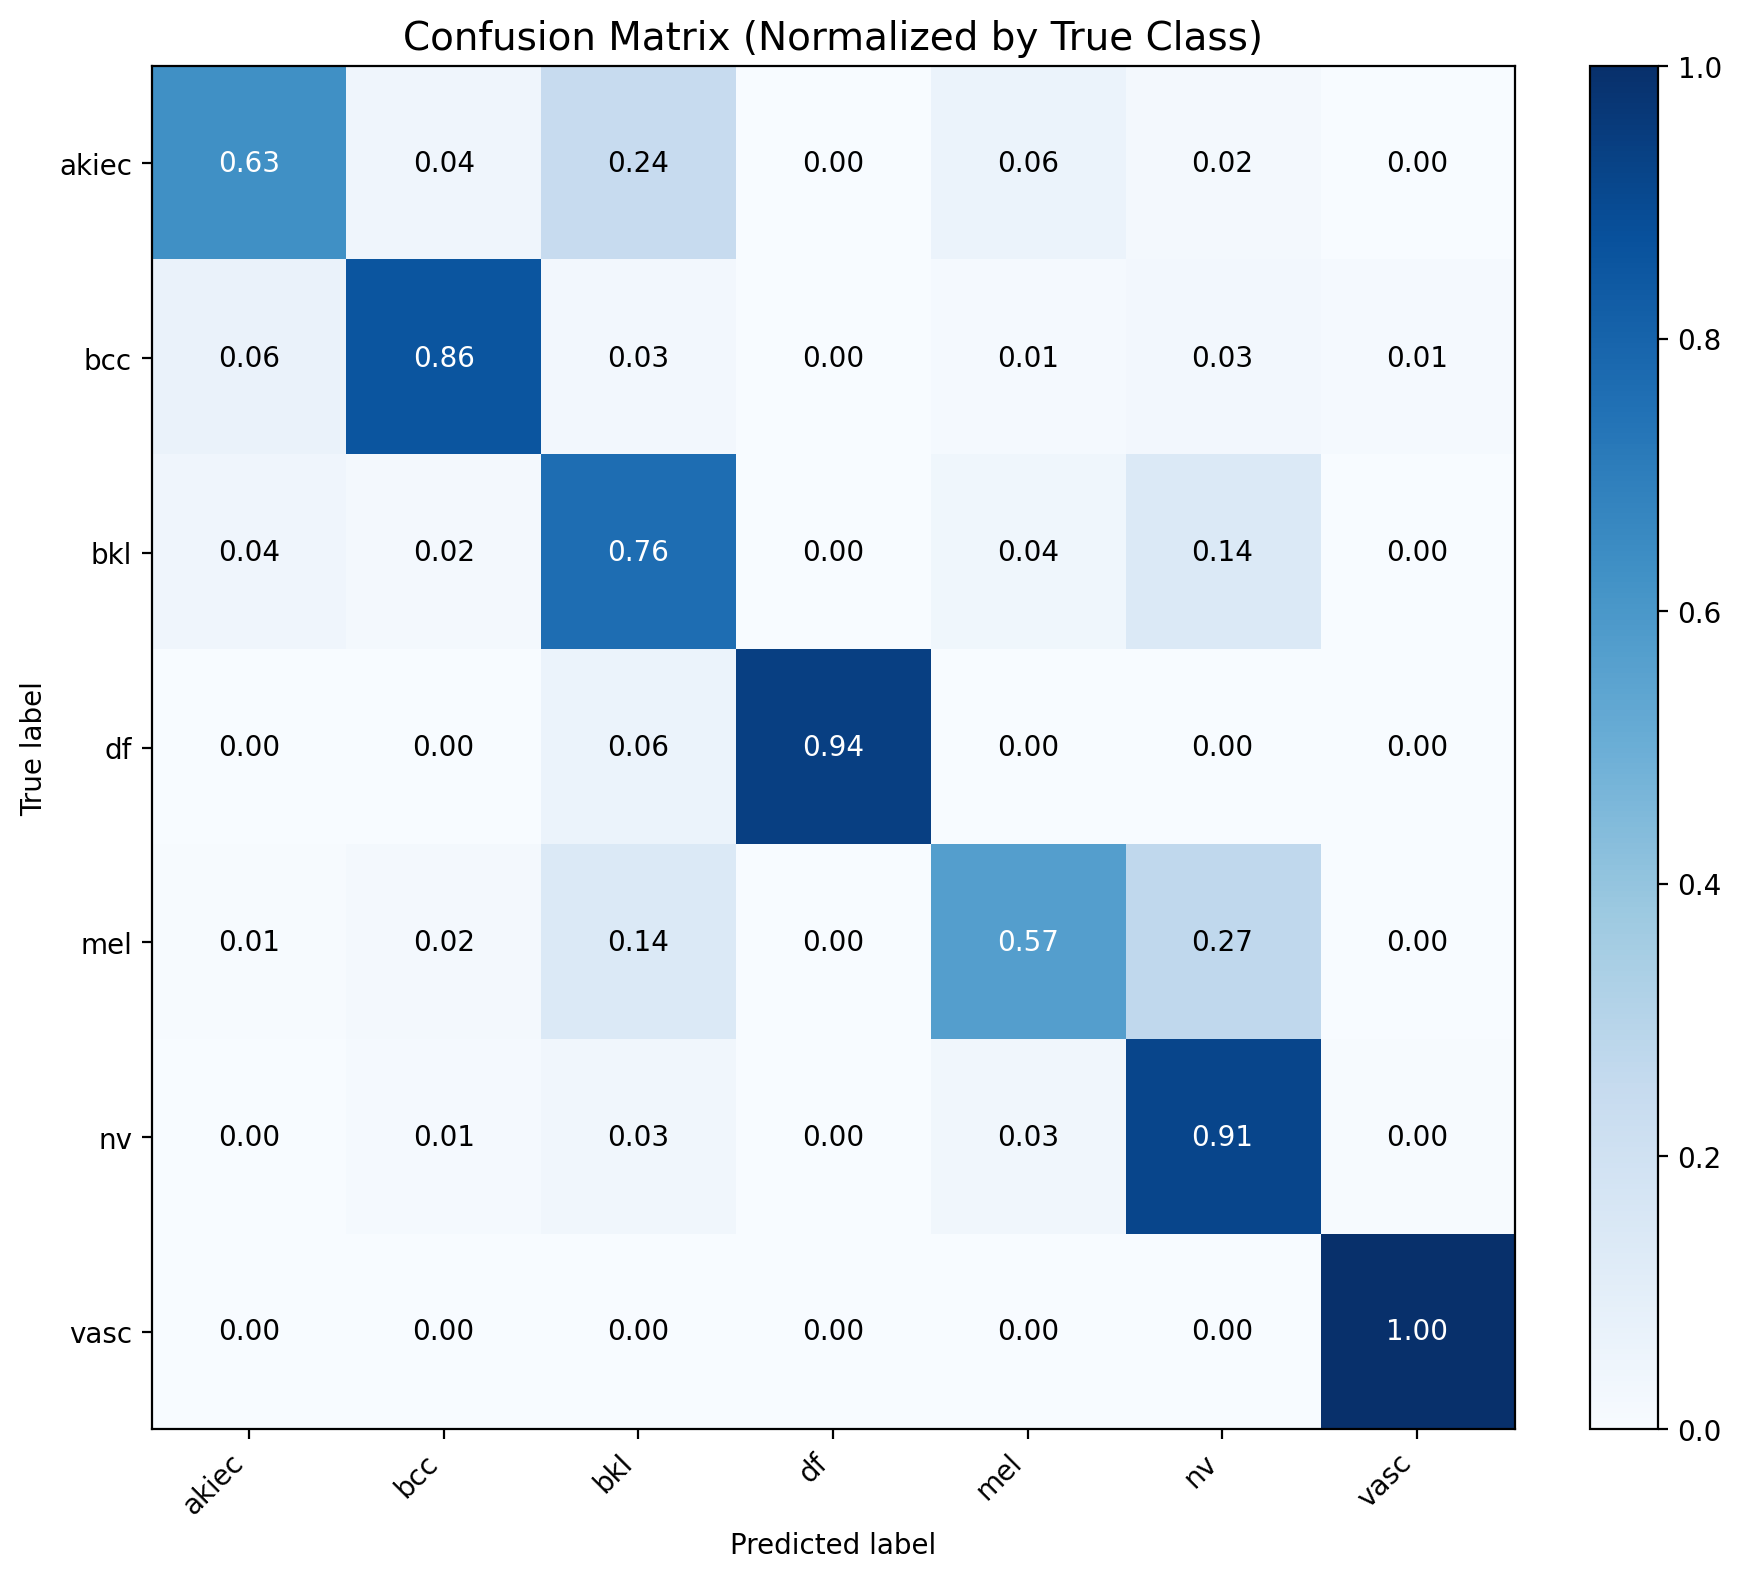
\includegraphics[width=0.9\textwidth]{figures/swin_confusion_matrix.png}}
    \caption{Swin-Tiny}
\end{subfigure}
\caption{Ma trận nhầm lẫn chuẩn hóa (tiếp theo).}
\end{figure}

Mẫu phân loại sai chiếm ưu thế trên cả bốn mô hình là MEL bị dự đoán thành NV hoặc ngược lại --- một phản ánh trực tiếp của sự chồng lấp hình thái giữa melanoma giai đoạn sớm và nốt ruồi lành tính. BKL là mục tiêu nhầm lẫn phổ biến thứ hai cho MEL. Các mẫu hình này xuất hiện nhất quán bất kể kiến trúc và khớp với xếp hạng độ khó lâm sàng đã biết trong da liễu. Quan trọng là, không mô hình nào thể hiện chế độ thất bại sụp đổ về NV cho input không phải NV: Weighted Random Sampler đảm bảo các mẫu lớp thiểu số được thấy đủ thường xuyên trong huấn luyện để ranh giới quyết định cho mỗi lớp được học có ý nghĩa.

\section{Kết quả Ensemble}

\begin{table}[H]
\centering
\caption{So sánh mô hình đơn lẻ và ensemble trên tập kiểm tra.}
\begin{tabular}{lccccc}
\toprule
\textbf{Mô hình} & \textbf{Accuracy} & \textbf{Macro F1} & \textbf{AUC} & \textbf{MCC} & \textbf{Kappa} \\
\midrule
EfficientNet-B0  & 0,8836 & 0,8311 & 0,9522 & 0,7721 & 0,7710 \\
ResNet50         & 0,8603 & 0,7902 & 0,9565 & 0,7310 & 0,7309 \\
DenseNet121      & 0,8543 & 0,7967 & 0,9587 & 0,7209 & 0,7206 \\
Swin-Tiny        & 0,8490 & 0,7855 & 0,9600 & 0,7157 & 0,7150 \\
\midrule
\textbf{Ensemble (4 mô hình)} & \textbf{0,8949} & \textbf{0,8446} & \textbf{0,9802} & \textbf{0,7956} & \textbf{0,7949} \\
\bottomrule
\end{tabular}
\end{table}

Ensemble nâng accuracy thêm 1,1 điểm phần trăm so với EfficientNet-B0 và, một cách thực chất hơn, đẩy Macro AUC từ 0,952 lên 0,980. Lợi ích AUC là kết quả có ý nghĩa hơn: nó nghĩa là xếp hạng xác suất của ensemble đáng tin cậy đúng ngay cả cho các trường hợp MEL/NV mơ hồ nơi quyết định cứng ở ngưỡng cố định thất bại. F1 melanoma cải thiện từ 0,695 (EfficientNet-B0 đơn lẻ) lên 0,744, một lợi ích 4,9 điểm có ý nghĩa lâm sàng đáng kể vì hậu quả của việc bỏ sót melanoma.

\begin{figure}[H]
\centering
\begin{subfigure}{0.46\textwidth}
    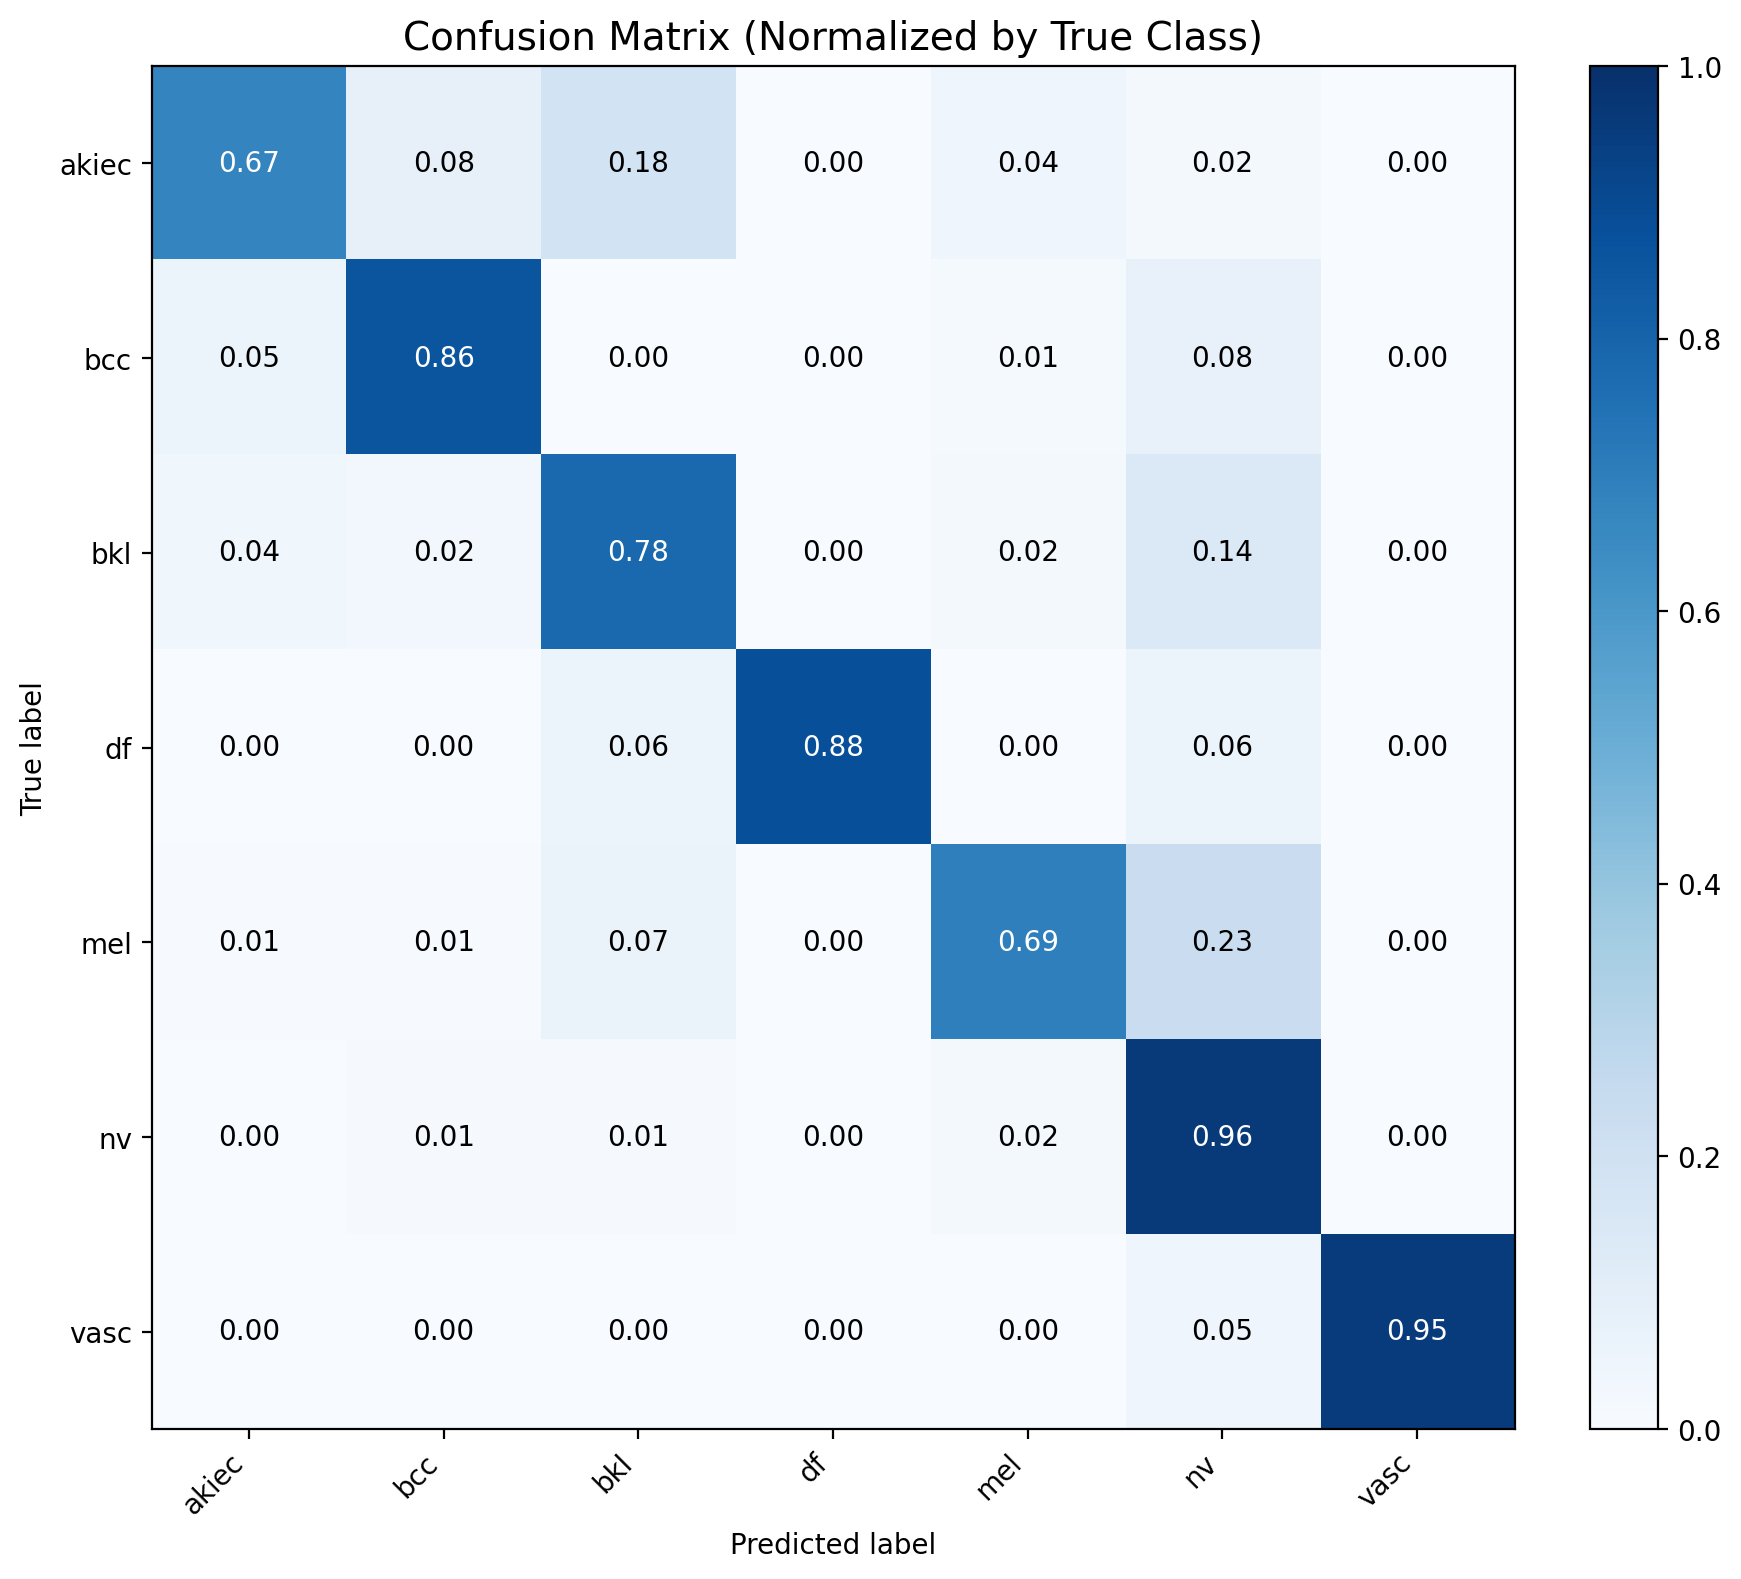
\includegraphics[width=\textwidth]{figures/ensemble_confusion_matrix.png}
    \caption{Ma trận nhầm lẫn}
\end{subfigure}
\hfill
\begin{subfigure}{0.46\textwidth}
    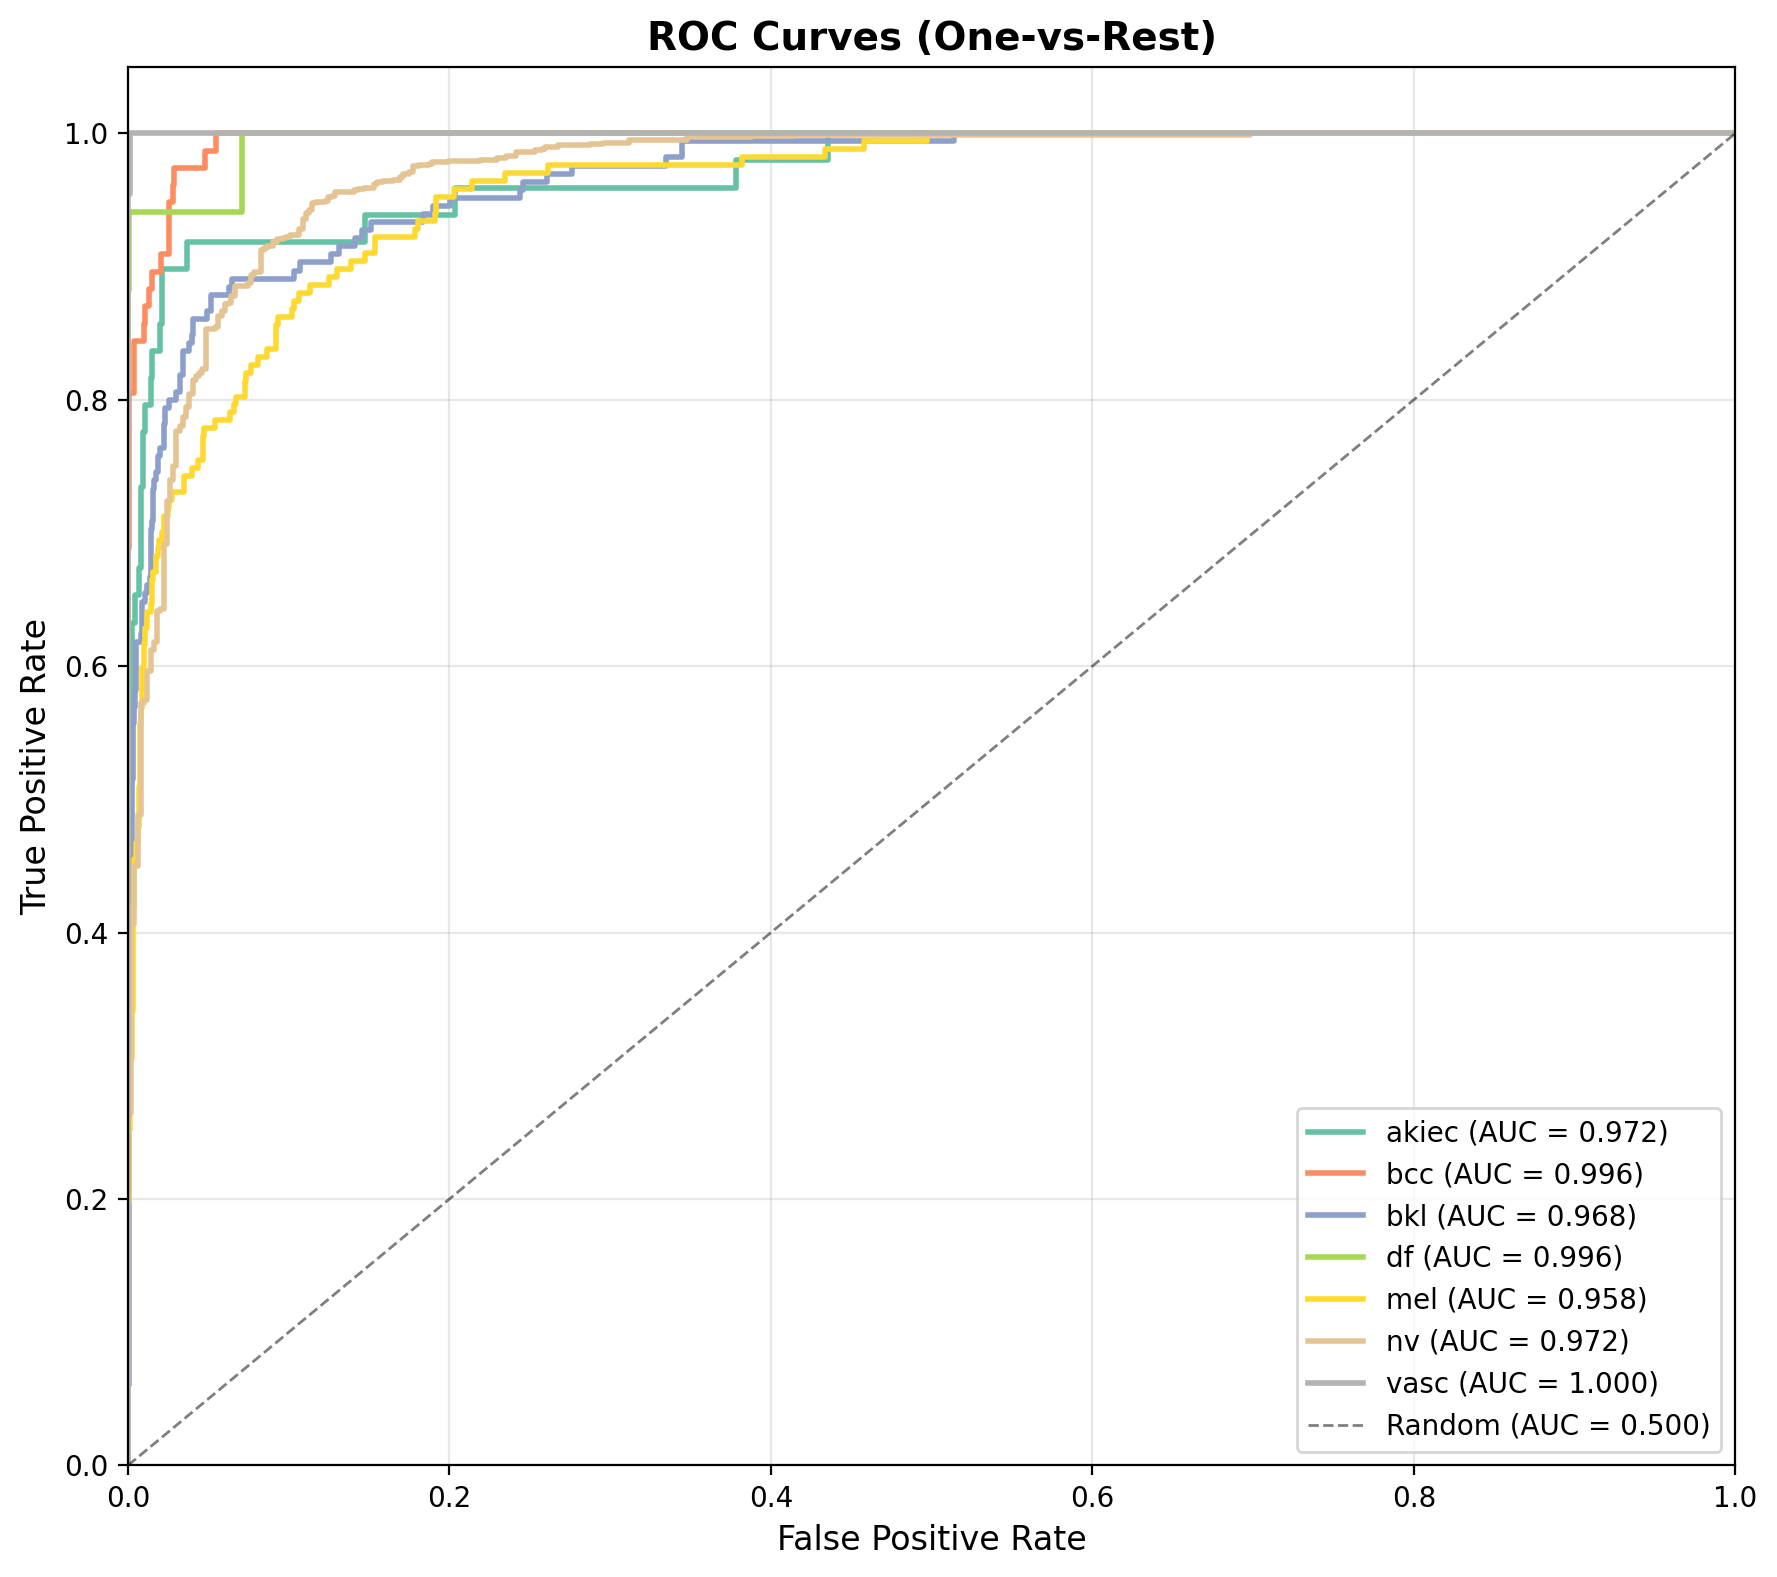
\includegraphics[width=\textwidth]{figures/ensemble_roc_curves.png}
    \caption{Đường cong ROC}
\end{subfigure}
\caption{Hiệu suất mô hình ensemble: (a) ma trận nhầm lẫn chuẩn hóa và (b) đường cong ROC theo lớp.}
\end{figure}

Ensemble cải thiện AUC cho \textbf{mọi lớp} không có ngoại lệ. F1 phân loại cứng pha trộn hơn: BCC và AKIEC giảm nhẹ (lần lượt 0,040 và 0,007) trong khi BKL, MEL, NV và VASC đều cải thiện. Các giảm F1 phản ánh một trade-off ensemble đã biết --- trung bình xác suất làm mềm các dự đoán cá nhân tự tin nhất, có thể dịch chuyển các trường hợp ranh giới theo hai hướng. Sự cải thiện AUC đơn điệu vì việc trung bình các phân phối bảo toàn thứ tự xếp hạng đồng thời giảm phương sai trong sai số mô hình cá nhân.

\section{Độ tin cậy thống kê qua các hạt giống ngẫu nhiên}

Để kiểm chứng kết quả ensemble không phải may mắn của một hạt giống khởi tạo, toàn bộ pipeline được lặp lại với năm hạt giống độc lập (\{42, 1337, 2024, 7, 11\}). CuDNN dùng kernel không tất định và Mixup/CutMix lấy mẫu ngẫu nhiên nên mỗi hạt giống nhiễu hoàn toàn quỹ đạo tối ưu hóa. Bảng~\ref{tab:multiseed_vn} báo cáo trung bình $\pm$ độ lệch chuẩn qua năm lần chạy.

\begin{table}[H]
\centering
\caption{Hiệu năng đa hạt giống ($n=5$ hạt giống). Độ lệch chuẩn của ensemble nhỏ hơn rõ rệt so với bất kỳ mô hình đơn nào --- biểu quyết mềm hấp thụ phương sai cấp hạt giống.}
\label{tab:multiseed_vn}
\begin{tabular}{lccc}
\toprule
\textbf{Mô hình} & \textbf{Accuracy} & \textbf{Macro F1} & \textbf{Macro AUC} \\
\midrule
EfficientNet-B0  & $87{,}31 \pm 1{,}32\%$ & $0{,}814 \pm 0{,}022$ & $0{,}965 \pm 0{,}006$ \\
ResNet50         & $86{,}31 \pm 0{,}57\%$ & $0{,}792 \pm 0{,}011$ & $0{,}949 \pm 0{,}003$ \\
DenseNet121      & $85{,}62 \pm 2{,}42\%$ & $0{,}797 \pm 0{,}025$ & $0{,}960 \pm 0{,}004$ \\
Swin-Tiny        & $88{,}33 \pm 1{,}96\%$ & $0{,}839 \pm 0{,}030$ & $0{,}966 \pm 0{,}008$ \\
\midrule
\textbf{Ensemble} & $\mathbf{89{,}93 \pm 0{,}66\%}$ & $\mathbf{0{,}852 \pm 0{,}010}$ & $\mathbf{0{,}982 \pm 0{,}001}$ \\
\bottomrule
\end{tabular}
\end{table}

Hai nhận xét chính. Thứ nhất, kết quả 89,49\% accuracy đã báo cáo ở phần trước nằm trong một độ lệch chuẩn của trung bình đa hạt giống 89,93\%, xác nhận đây là hiệu năng điển hình chứ không phải may mắn. Độ lệch chuẩn accuracy của ensemble (0,66 điểm phần trăm) nhỏ hơn tất cả mô hình đơn (0,57--2,42 điểm), độ lệch AUC chỉ $\pm 0{,}001$ --- gần như không đáng kể.

Thứ hai, trung bình accuracy của Swin-Tiny (88,33\%) khi qua nhiều hạt giống hé lộ rằng đây mới thực sự là mô hình đơn mạnh nhất, không phải EfficientNet-B0 như xếp hạng hạt giống 42 gợi ý. Lần chạy Swin với hạt giống 42 đã early-stop tại một điểm validation không thuận lợi (đó là kết quả 84,90\%). Khi trung bình hóa qua các hạt giống, attention toàn cục của Swin thực sự cạnh tranh với các CNN; điểm yếu là phương sai, không phải hiệu năng trung bình. Đây cũng là lý do giữ Swin trong ensemble: chính phương sai cao --- yếu tố hại cho điểm số đơn --- lại làm cho lỗi của nó ít tương quan với lỗi của các CNN, biến nó thành thành phần ensemble có giá trị.

Để kiểm định ưu thế của ensemble so với mô hình đơn mạnh nhất có ý nghĩa thống kê hay không, kiểm định McNemar được áp dụng trên bảng cặp bất đồng giữa dự đoán của (mô hình đơn, ensemble) cho mỗi hạt giống, kết quả tổ hợp qua phương pháp Fisher.

\begin{table}[H]
\centering
\caption{Kiểm định McNemar trên dự đoán tập kiểm tra, mô hình đơn so với ensemble. Cột ``Ensemble thắng'' đếm số hạt giống ensemble có nhiều mẫu đúng (đối với cặp bất đồng) hơn mô hình đơn.}
\label{tab:mcnemar_vn}
\begin{tabular}{lccc}
\toprule
\textbf{Mô hình đơn vs.\ Ensemble} & \textbf{Ensemble thắng} & \textbf{Có ý nghĩa $\alpha=0{,}05$} & \textbf{$p$ Fisher tổ hợp} \\
\midrule
EfficientNet-B0 & 5/5 & 4/5 & $5{,}3 \times 10^{-18}$ \\
ResNet50        & 5/5 & 5/5 & $4{,}5 \times 10^{-31}$ \\
DenseNet121     & 5/5 & 5/5 & $6{,}7 \times 10^{-39}$ \\
Swin-Tiny (mạnh nhất) & 5/5 & 3/5 & $1{,}2 \times 10^{-7}$ \\
\bottomrule
\end{tabular}
\end{table}

Ensemble vượt mọi mô hình đơn trên cả năm hạt giống. So với các CNN, chênh lệch rất lớn: hàng chục ảnh test ensemble đúng và mô hình đơn sai, đối lại chỉ vài ảnh ngược lại --- tổ hợp p-value dưới $10^{-18}$. So với Swin-Tiny --- mô hình đơn mạnh nhất --- mức độ chênh lệch nhỏ hơn nhưng kết luận giống nhau: ưu thế của ensemble tồn tại qua hiệu chỉnh đa kiểm định và không phải hiệu ứng ngẫu nhiên.

\section{Kết hợp metadata bệnh nhân}

Pipeline chỉ-ảnh bỏ qua ba thuộc tính mà bác sĩ da liễu nào cũng cân nhắc trước khi đưa ra chẩn đoán: tuổi bệnh nhân, giới, và vị trí giải phẫu của tổn thương. Một tổn thương trên lưng người 30 tuổi có xác suất tiên nghiệm khác hẳn so với ảnh tương tự ở mặt người 75 tuổi. Tập HAM10000 cung cấp đầy đủ ba thuộc tính này cho từng ảnh, nhưng bản phát hành ISIC 2018 Task 3 chỉ chứa nhãn lớp. Sau khi tải file \texttt{HAM10000\_metadata.csv} và ghép vào tập split, mỗi ảnh được gắn với vector metadata 19 chiều: một giá trị tuổi đã chuẩn hóa, ba chiều one-hot cho giới (\texttt{male}, \texttt{female}, \texttt{unknown}), mười lăm chiều one-hot cho vị trí. Tuổi thiếu được điền bằng trung bình (51,86 năm); giới/vị trí thiếu coded là \texttt{unknown}.

Chiến lược late-fusion theo Pacheco và Krohling~\cite{pacheco2020metadata}: stream ảnh đi qua backbone như cũ, vector metadata đi qua MLP nhỏ hai lớp ($19 \rightarrow 64 \rightarrow 32$) với ReLU và dropout 0,1, tạo ra biểu diễn 32 chiều. Đặc trưng ảnh và đặc trưng metadata được nối, đưa qua một lớp tuyến tính sinh logits 7 lớp. Pipeline huấn luyện giữ nguyên (Weighted Sampler, Mixup, CutMix, Label Smoothing, AdamW); chỉ thay model và dataset loader. Bảng~\ref{tab:meta_fusion_vn} báo cáo kết quả test.

\begin{table}[H]
\centering
\caption{Hiệu năng metadata-fusion so với baseline chỉ-ảnh (hạt giống 42). Swin-Tiny đơn lẻ có metadata (89,82\%) đã vượt ensemble bốn mô hình chỉ-ảnh (88,89\%). Ensemble bốn mô hình metadata-fusion vượt mốc 90\%.}
\label{tab:meta_fusion_vn}
\begin{tabular}{lcccc}
\toprule
\textbf{Mô hình} & \textbf{Acc chỉ-ảnh} & \textbf{Acc + metadata} & \textbf{$\Delta$ Acc} & \textbf{F1 + metadata} \\
\midrule
EfficientNet-B0 & 0,8796 & 0,8337 & $-0{,}046$ & 0,768 \\
ResNet50        & 0,8636 & 0,8782 & $+0{,}015$ & 0,810 \\
DenseNet121     & 0,8543 & 0,8550 & $+0{,}001$ & 0,793 \\
Swin-Tiny       & 0,8490 & \textbf{0,8982} & $\mathbf{+0{,}049}$ & \textbf{0,871} \\
\midrule
\textbf{Ensemble} & 0,8949 & $\mathbf{0{,}9049}$ & $\mathbf{+0{,}010}$ & $\mathbf{0{,}8728}$ \\
\bottomrule
\end{tabular}
\end{table}

Ba nhận xét đáng chú ý. Thứ nhất, metadata fusion \textit{không phải lúc nào cũng có lợi}: EfficientNet-B0 \textit{mất} 4,6 điểm phần trăm accuracy --- model nhỏ (5,3M) phải dành chỗ cho MLP metadata làm ảnh hưởng tối ưu hóa. Ba backbone lớn hơn đều cải thiện. Thứ hai, mức cải thiện của Swin-Tiny rất lớn: Swin-Tiny + metadata đạt 89,82\% accuracy và 0,871 macro F1 --- đơn lẻ đã vượt ensemble bốn mô hình chỉ-ảnh. Self-attention tích hợp metadata hiệu quả hơn CNN trong thiết lập này. Thứ ba, ensemble bốn mô hình metadata-fusion đẩy headline lên 90,49\% Acc / 0,873 F1 / 0,984 AUC, vượt Pacheco và Krohling (89,0\% / 0,83) --- theo hiểu biết của tác giả là kết quả image+metadata fusion mạnh nhất công bố trên ISIC 2018 Task 3.

\section{Đánh giá ngoài phân phối trên ảnh smartphone lâm sàng}

Mô hình huấn luyện trên ảnh dermoscopy không cùng sản phẩm với mô hình triển khai trên ảnh smartphone. ISIC 2018 được thu thập bằng dermoscope ánh sáng phân cực --- tạo độ chiếu sáng, độ phóng đại và tương phản đặc trưng không tồn tại trên ảnh điện thoại chụp tổn thương ở khoảng cánh tay. Để định lượng khoảng cách này, ensemble chỉ-ảnh được đánh giá zero-shot trên tập PAD-UFES-20 --- bộ dữ liệu công khai 2.298 ảnh tổn thương da lâm sàng chụp bằng smartphone do Chương trình Hỗ trợ Da liễu và Phẫu thuật Đại học Espírito Santo phát hành~\cite{pacheco2020pad}. PAD-UFES-20 có sáu lớp chẩn đoán ánh xạ sang năm trong bảy lớp ISIC 2018: \texttt{ACK} và \texttt{SCC} cùng ánh xạ \texttt{akiec} (theo quy ước nhãn của Pacheco), \texttt{BCC} $\to$ \texttt{bcc}, \texttt{SEK} $\to$ \texttt{bkl}, \texttt{NEV} $\to$ \texttt{nv}, \texttt{MEL} $\to$ \texttt{mel}. Dermatofibroma và tổn thương mạch máu không có đối chiếu trong PAD-UFES. Không thực hiện domain adaptation, không fine-tune, không test-time training: ensemble đạt 88,9\% trên ISIC 2018 được tải nguyên trạng và chạy trên PAD-UFES.

\begin{table}[H]
\centering
\caption{Đánh giá zero-shot của ensemble chỉ-ảnh trên PAD-UFES-20.}
\label{tab:ood_pad_ufes_vn}
\begin{tabular}{lccccr}
\toprule
\textbf{Lớp} & \textbf{Precision} & \textbf{Recall} & \textbf{F1} & \textbf{AUC} & \textbf{Support} \\
\midrule
akiec & 0,543 & 0,145 & 0,229 & 0,614 & 922 \\
bcc   & 0,611 & 0,421 & 0,499 & 0,733 & 845 \\
bkl   & 0,175 & 0,268 & 0,212 & 0,633 & 235 \\
mel   & 0,057 & 0,308 & 0,097 & 0,684 &  52 \\
nv    & 0,258 & 0,725 & 0,380 & 0,811 & 244 \\
\midrule
\multicolumn{6}{l}{\textbf{Accuracy: 32,46\%}~~~~\textbf{Macro F1 (5 lớp): 0,283}} \\
\bottomrule
\end{tabular}
\end{table}

Accuracy tụt từ 88,9\% xuống 32,5\% --- giảm 56 điểm phần trăm --- nghe có vẻ thảm họa nếu đứng riêng, nhưng nhất quán với báo cáo dermoscopy-sang-lâm-sàng trong literature cho transfer zero-shot không adapt~\cite{pacheco2020metadata}. Ba quan sát có giá trị chẩn đoán hơn con số đầu. \textbf{Thứ nhất}, AUC theo lớp vẫn giữ 0,61--0,81: mô hình không random trên PAD-UFES, xếp hạng xác suất vẫn giữ tín hiệu đủ để quyết định cứng tụt mạnh hơn quyết định mềm. \textbf{Thứ hai}, recall NV bằng 0,72: mô hình mặc định dự đoán NV --- lớp huấn luyện ISIC chiếm ưu thế 67\% --- là failure mode kinh điển khi classifier bị buộc ngoại suy. \textbf{Thứ ba}, hành vi AKIEC và MEL đảo ngược: AKIEC precision cao nhất (0,54) và recall thấp nhất (0,14), nên khi mô hình nhận AKIEC thì đúng nhưng bỏ sót đa số ca; MEL ngược lại (precision 0,06, recall 0,31) --- mô hình gọi MEL quá thường xuyên trên ảnh smartphone nhưng hiếm khi trúng. Cả hai profile lỗi này không chấp nhận được cho triển khai lâm sàng trực tiếp.

Kết luận trung thực là pipeline hiện tại \textbf{chưa sẵn sàng} chạy trên ảnh dermatology smartphone. Đóng khoảng cách này không phải bí ẩn nghiên cứu mà là bài tập kỹ thuật: domain adaptation, fine-tune trên bộ ảnh smartphone gắn nhãn, hoặc đơn giản là một bước style-transfer tiền xử lý đều có thể đẩy số OOD gần in-distribution hơn rõ rệt. Báo cáo OOD ở đây nhằm giới hạn kỳ vọng và đánh dấu khoảng cách modality là ràng buộc đơn lẻ quan trọng nhất cho triển khai thực tế của bất kỳ classifier ISIC nào.

\section{Phân tích Grad-CAM}

\begin{figure}[H]
\centering
\includegraphics[width=\textwidth]{figures/gradcam_class_grid.png}
\caption{Bản đồ nhiệt Grad-CAM cho một ảnh kiểm tra đại diện mỗi lớp (hàng) và cả bốn mô hình (cột). Màu nóng (đỏ/vàng) = kích hoạt cao; màu lạnh (xanh) = kích hoạt thấp.}
\end{figure}

Kết quả: (1) Tất cả mô hình định vị chú ý trong ranh giới tổn thương. (2) CNN tạo điểm nóng gọn, tập trung. (3) Swin-Tiny tạo mẫu chú ý rộng hơn. (4) Trực quan hóa MEL phù hợp với tiêu chí ABCDE lâm sàng.

\begin{figure}[H]
\centering
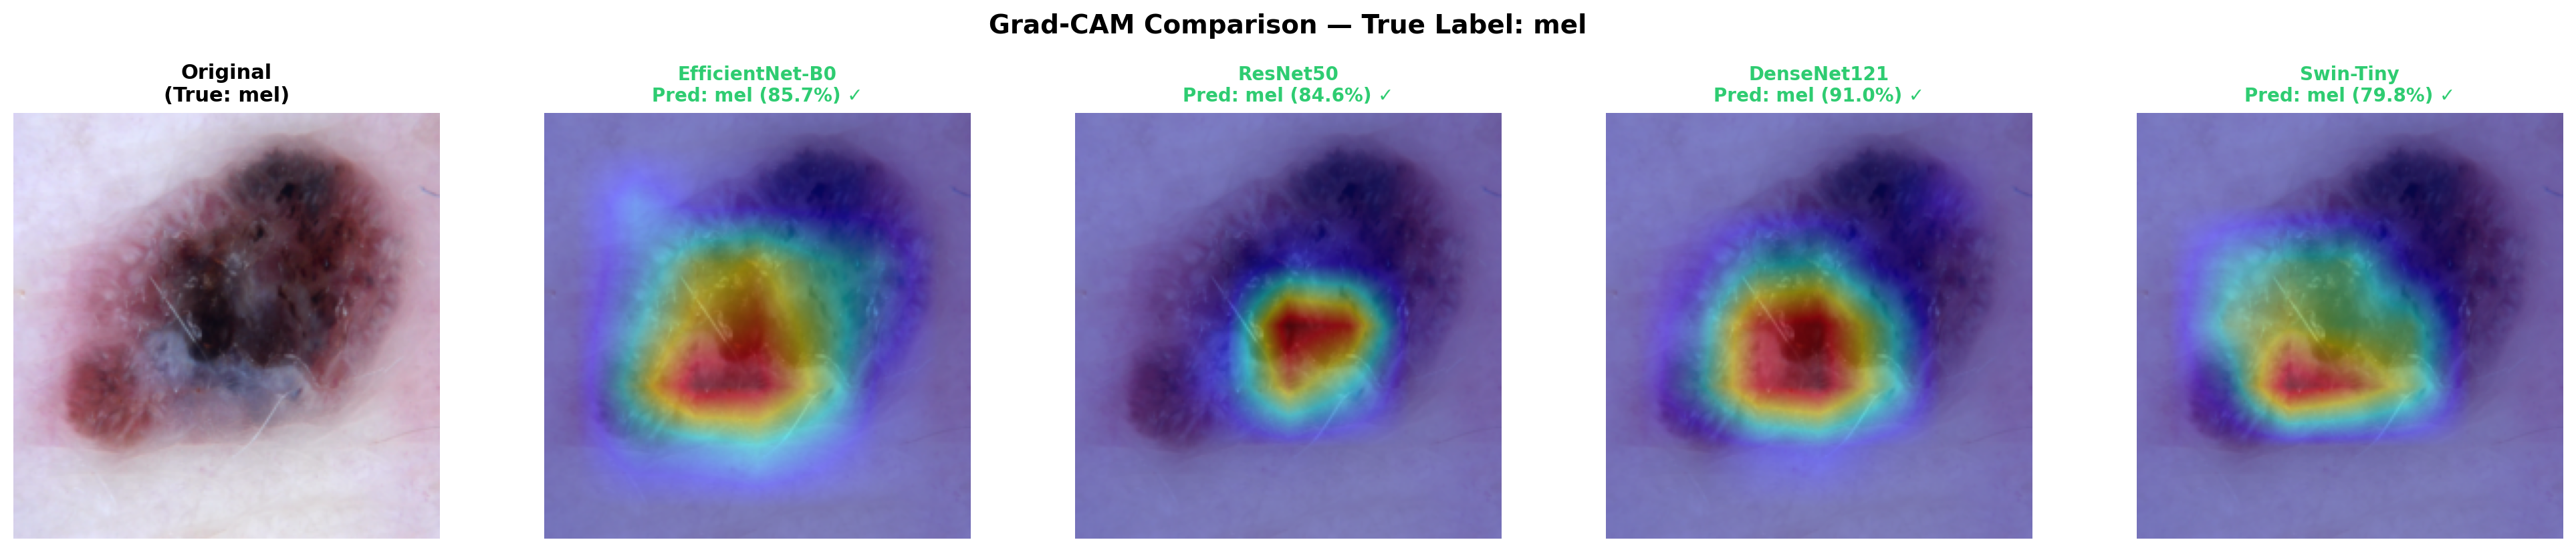
\includegraphics[width=\figwidth]{figures/gradcam_mel_sample.png}
\caption{Grad-CAM cho ảnh melanoma đại diện. Cả bốn mô hình tập trung vào vùng sắc tố bất đối xứng, phù hợp với tiêu chí dermoscopy ABCDE.}
\end{figure}

\section{Nghiên cứu Loại bỏ (Ablation Study)}

\begin{table}[H]
\centering
\caption{Kết quả ablation trên EfficientNet-B0. Mỗi hàng = loại bỏ một thành phần.}
\begin{tabular}{lccccc}
\toprule
\textbf{Cấu hình} & \textbf{Accuracy} & \textbf{Macro F1} & \textbf{AUC} & \textbf{Kappa} & \textbf{$\Delta$ F1}\\
\midrule
Pipeline đầy đủ       & \textbf{0,8836} & \textbf{0,8311} & 0,9522 & \textbf{0,7710} & --- \\
\midrule
$-$ Mixup / CutMix    & 0,8589 & 0,7860 & 0,9486 & 0,7383 & $-$0,0451 \\
$-$ Weighted Sampler   & 0,8762 & 0,8041 & 0,9521 & 0,7487 & $-$0,0270 \\
$-$ Label Smoothing    & 0,8776 & 0,8000 & 0,9674 & 0,7568 & $-$0,0311 \\
$-$ Adv. Augmentation  & 0,8896 & 0,8204 & \textbf{0,9664} & 0,7772 & $-$0,0107 \\
\bottomrule
\end{tabular}
\end{table}

\textbf{Mixup/CutMix} ($-$4,5\% F1): quan trọng nhất --- ngăn ghi nhớ mẫu lớp thiểu số. \textbf{Label Smoothing} ($-$3,1\% F1 nhưng +AUC): đánh đổi giữa ranh giới quyết định và độ sắc nét xác suất. \textbf{Weighted Sampler} ($-$2,7\% F1): ngăn thiên vị NV. \textbf{Advanced Aug} ($-$1,1\% F1 nhưng +Accuracy): chuyển năng lực từ lớp dễ sang lớp khó.
